\newgeometry{textwidth=16cm}
\chapter[Modélisation des interactions intermoléculaires]{Modélisation des interactions intermoléculaires}
\minitoc
\restoregeometry

\newpage

\section*{Introduction}
\markright{INTRODUCTION}{}

Les interactions non-covalentes ou interactions Van der Waals occupent une place prépondérante dans les problématiques actuelles de recherche, celles-ci étant aujourd'hui considérées comme les pierres angulaires de disciplines telles que la chimie supramoléculaire, la science des matériaux ou la biochimie.  Après les liaison hydrogènes et les interactions électrostatiques fortes (\textit{e.g.} charge- charge, charge- dipôle, dipôle- dipôle), la plus significatif interaction non covalente est probablement laquelle implique les systèmes aromatiques \cite{grimme2008special}. Attractives interactions entre cycles aromatiques ont été considérées comme  responsables de la stabilité de la double hélice d'ADN et ARN, ainsi comme l'agrégation de Porphyrines \cite{mcgaughey1998pi}.

L'énergie d'interaction intermoléculaire d'un ensemble de molécules se situe généralement entre 1 et 20 kcal/mol selon le nombre et le type de molécules impliquées. Cependant, l'énergie d'une liaison chimique covalente se mesure entre 100 et 300 kcal/mol, ce qui est d’un autre ordre de grandeur. De même, la portée d’une liaison chimique dépasse rarement quelques Angströms tandis que les interactions intermoléculaires s'étendent théoriquement jusqu'à l'infini (électrostatique) et de manière pratique entre 2 et 10 Angströms selon la taille et la nature du système.

Malgré toute cette importance pour grandes structures, $\pi$-stacking est un phénomène pas bien connu. L’étude expérimentale de ces interactions présente un défi car il est complique séparer les interactions $\pi$-stacking d’interactions secondaires ou les effets de solvant. A cause de ces difficultés expérimentales, les études en chimique computationnelle apparaissent ainsi qu’un avantage pour comprendre la nature fondamentale des interactions non covalentes, et l’influence sur les systèmes chimiques. 

\newpage

\section{Bases Théoriques}

La modélisation en chimique théorique de la corrélation électronique représente la principale difficulté dans les systèmes des molécules ou bien dans de complexes faisant intervenir des interactions intermoléculaires. Ce phénomène déterminé par l’impossibilité de trouver deux électrons au même endroit de l’espace, apparaît puisque il n’existe pas une solution analytique à l’équation de  Schrödinger à des systèmes à plus d’un électron; plusieurs méthodes ont été développées pour traites des systèmes électroniques à n corps.\\

La méthode Hartree-Fock, proposée indépendamment par Hartree et Fock en 1930 \cite{slater1930note}, met chaque électron d’un systèmes dans un champ moyen de façon isolé, dans lequel chaque électron pris subit l’interaction des n-1 autres électrons du systèmes. La méthode permet de reproduire le trou de Fermi, par contre ne prends pas compte de trou de Coulomb et il manque de la corrélation électronique, indispensable pour calculer avec la précision nécessaire des énergies et différences. Cela sera ajouté par perturbation, interaction de configurations, random phase approximation ou autres méthodes post Hartree-Fock.\\

L’énergie d’interaction intermoléculaire est une observable qu’on peut interpréter par différentes décompositions qui ont un sens physique. Buckingham \cite{buckingham1967permanent}, a proposé par exemple une décomposition de l’énergie d’interaction intermoléculaire en quatre grandes contributions : l’électrostatique $E_{elec}$, l’induction $E_{ind}$, l’echange-repulsion $E_{rep}$, et la dispersion $E_{disp}$.\\

\begin{equation}
\Delta E = E_{elec} + E_{ind} + E_{rep} + E_{disp}
\end{equation} 

L’interaction électrostatique est l’ensemble des interactions coulombiennes des deux densités de charges isolées, est additive et peut être répulsive ou attractive selon l’orientation relative des molécules. Elle constitue la plus grande partie de l’interaction intermoléculaire.  
L’énergie d’induction est la stabilisation d’un système par la polarisation des constituant par le champ électrique qu’ils subissent de la part de densités de charge que les avoisinant. Cette énergie est non additive et toujours attractive.\\

La répulsion vient du principe de Pauli, qui stipule que deux électrons ne peuvent pas occuper le même spin au sein d’une même orbitale. C’est une interaction toujours répulsive et qui apparaît seulement à court distance.\\

Finalement la dispersion n’a pas d’équivalent classique car c’est une interaction qui est liée à la corrélation électronique de deux densités de charge en interaction. Elle est attractive et existe dans tous les complexes.\\

Il y a deux manière différentes de calculer une énergie d’interaction intermoléculaire. L’une est la méthode supermoléculaire, et l’autre est la construction d’une interaction par contributions directement résultat des fonctions d’onde des monomères séparés.Dans la méthode supermoleculaire l’énergie d’interaction intermoléculaire est la différence entre l’énergie totale du dimère et la somme de l’énergie total de chaque monomère.


\begin{equation}
\Delta E = E_{AB} - E_{A} - E_{B} \label{eq2}
\end{equation}

A et B représentent les monomères et AB le dimère. Dans ce cas là, une erreur subtile peut se produire autour de l’énergie d’interaction. Cette erreur est connue sous le nom de Basis Set Superposition Error (BSSE) \cite{sherrill2010counterpoise}. Si nous calculons les deux monomères dans leurs bases spécifiques, et ensuite un dimère dans l’ensemble des fonctions de base des monomères, nous pourrons utiliser les orbitales virtuelles d’un monomère pour agrandir la base disponible pour la distribution de charge de l’autre monomère et vice versa. Le résultat est donc une augmentation de la qualité de la base pour le dimère vis-à-vis des monomères, et par conséquent une surestimation de l’énergie de l’interaction. Pour corriger l’erreur de BSSE, une méthode possible est de travailler dans une base complète ou saturée pour les monomères et le dimère. Une autre méthode est de calculer l’énergie des monomères dans la base du dimère, ce qui est le plus fréquemment utilisé sous le nom de counterpoise grace a Boys et Bernardi \cite{boys1970calculation}. Cette correction entraîne que pour chaque distance intermoléculaire considérée il faut calculer l’énergie totale du dimère et des monomères.\\

L'energie sans correction donnée pour l'equation \ref{eq2}  peut-être modifiée pour l'estimation de la quantité pour laquelle le monomère A est stabilisé artificiellement pour la base supplémentaire du monomère B et vice versa, avec la relation suivante:

\begin{equation}
E_{BASE}(A) = E_{A}^{AB}(A) - E_{A}^{A}(A)
\end{equation}

\begin{equation}
E_{BSSE}(B) = E_{B}^{AB}(B) - E_{B}^{B}(B)
\end{equation}

Où l'exposant désigne la base utilisée, l'indice désigne la géométrie et le symbole entre parenthèses est le système chimique considéré Ainsi nous soustrayons l'énergie du monomère A et ses bases de l'énergie et bases du dimer, également dans le cas du monomère B.\\

Pour le moment nous considérons que la géométrie des monomères ne changent pas quand ils s'approchent pour former le complexe . Normalement cette approximation simplifie les calculs et donne de bon résultat.\\

Le calcul direct d’une énergie d’interaction par la méthode supermoléculaire ne donne aucune information sur la nature de l’interaction. Il y a des méthodes pour décomposer l’énergie d’interaction en différentes contributions ayant en sens physique.\\

La première théorie mécanique quantique pour interactions intermoléculaire a été développée en 1930 par London et al \cite{london1930z}, (la même idée été dégagée plutôt par Wang \cite{wang1927mutual}. Cette théorie est basée en le standard bas ordre de l’expansion  de perturbation de Rayleidgh Schrödinger avec l’hamiltonien non perturbé des monomères pas interagissant. La différence entre le totale et l’hamiltonien non perturbé est l’opérateur V d’interaction intermoléculaire, lequel est remplacé par ses multipôles expansions. La méthode de London est validée seule de façon asymptotique pour large séparation intermoléculaire.\\

Elle peut être améliorée par l’utilisation de l’opérateur \textbf{V} non étendu, l’expansion de perturbation résultant est  dénommée comme l’approximation de la polarisation. Les composant qui sont présentes dans la polarisation et qui manquent dans la théorie de London sont visé comme l’effet de pénétration.\\ 

Autre approche, la méthode de Morokuma, qui est l’une des premières méthodes développées, modifiée plus tard par Kitaura et Morokuma, où l'energie est divisée au niveau Hartree-Fock dans les composants  électrostatique, echange, polarisation et transfert de charge. Ces constituants sont determinés pour le change de l'energie totale quand quelques elements bien defini sont eliminés de la matrice d'interaction de Fock et la matrice de recouvrement. Ils derivent d'un fonction d'onde  qui n'a pas été antisymetrisé \cite{morokuma1977molecules}. Restricted Virtual Space (RVS), qui a été proposée indépendamment par Stevens et Fink \cite{stevens1987frozen}, corrige nombreux tendance insatisfaisant de la décomposition de Morokuma en conséquence des termes lesquels n’étaient pas bien corrigés du principe d’exclusion de Pauli. Cependant elle combine leurs termes électrostatique et d’échange et modifie l’évaluation de la polarisation et les composants de transfert de charge \cite{chen1996energy}.


\section{Interactions intermoléculaires en théorie des perturbations}


A partir de la théorie des perturbations de Rayleigh-Schr\"{o}dinger nous pouvons construire l'énergie d'interaction d'un système, puisque elles sont faibles. L'Hamiltonien du système est la somme de l'hamiltonien de chaque monomere $H^{A/B}$ dont on connait la solution plus un terme perturbatif V. 

\begin{equation}
H = H^{A} + H^{B} + V
\end{equation}

\begin{equation}
H = H_{0}^{A} + W^{A} + H_{0}^{B} + W^{B} + V
\end{equation}

Les termes $W^{A/B}$ représentent des perturbations intramoléculaire des monomères, connues par la corrélation normal de chaque fragment, et V représente la perturbation intermoléculaire.\\

Sans la corrélation nous avons $H_{0} = H^{A} + H^{B}$ avec $E_{0} = E^{A} + E^{B}$, ou V devient l'interaction electrostatique entre A et B. Nous ecrivons l'equation de Schr\"{o}dinger :

\begin{equation}
(H_{0} - E_{0}) \psi (\xi) = (E_{int} - \xi V) \psi (\xi)
\end{equation}

Avec le paramètre $\xi$ pour moduler la perturbation. La théorie de Rayleigh-Schr\"{o}dinger fournit une série de corrections pour l'energie et la fonction d'onde \cite{chipman1973perturbation}.

\begin{equation}
\psi = \phi_{0} + \sum_{n} \xi^{n} \phi_{pol}^{(n)}
\end{equation}

\begin{equation}
E_{pol}^{(n)} = \langle \phi_{0}|V| \phi_{pol}^{(n)}
\end{equation}

Le terme \og pol \fg{} signifie qu’on est dans l'approximation de polarisation, sans effet d'un échange d’électrons entre les monomères dans la fonction $\phi_{pol^{(0)}}$, violant ainsi le principe d’antisymétrie. Les orbitales ne sont ni orthogonalisées, ni relaxées, mais proviennent directement du calcul de monomères séparés.\\

Pour assurer la convergence de la fonction est employé une asymptote. 

\begin{equation}
E_{int} = \sum_{n=1}^{N} E_{pol}^{(n)} + O(1/R^{2 (N+1)})
\end{equation}

 Pour retrouver des termes classiques induction et dispersion, l'énergie en deuxième ordre est encore décomposé en deux parties selon les excitations impliquées, selon la figure \ref{figExc}.

\singlespacing
\begin{figure}[H]
	\centering
	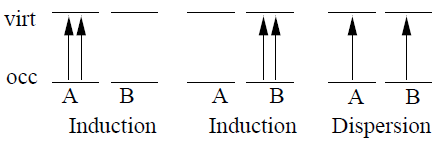
\includegraphics[scale=0.7]{image/D-I} \label{figExc}
	\caption[Les excitations contribuent à l'énergie
	de perturbation intermoléculaire en $2^{eme}$ ordre]{Classes d'excitations qui contribuent à l'énergie
		de perturbation intermoléculaire en $2^{eme}$ ordre}
\end{figure}



\section{La Théorie de Perturbations à Symétrie Adaptée (SAPT)}



Cette théorie est un ab initio méthode qui prends en compte les déficiences de la théorie de London et permet de calculer la surface énergie potentiel, grâce à une structure conceptuel pour comprendre le phénomène des interactions intermoléculaire.\\

Le point du départ est similaire à la théorie de London avec l'hamiltonien non perturbé, mais chacune des corrections à l’énergie d’interaction calculées dans cette approximation peuvent être classifiés tels en décrivant les quatre interactions fondamentales: l’électrostatique,  l’induction, l’échange et la dispersion. Ainsi SAPT représente l’énergie d’interactions comme la somme des termes bien définis avec interprétation physique.\\

Les propriétés de cette approximation ont été étudiées depuis 1960 pour systèmes simples comme H2+. Dans le cas de systèmes multiélectroniques SAPT a fallu appliquer une double perturbation, laquelle a été fait après 1970 \cite{szalewicz1979symmetry}.L’hamiltonien du dimère est partitionné dans les contributions de l’opérateur de Fock de chaque monomère (F), l’interaction entre les monomères (V) et le potentiel de fluctuation (W).

\begin{equation}
H = F_{A} + F_{B} + V + W_{A} + W_{B}
\end{equation}

L’énergie d’interaction peut être décrit comme une série perturbative :

\begin{equation}
E_{int} = \sum_{n=1}^{\infty} \sum_{k=0}^{\infty} \sum_{l=0}^{\infty} (E_{pol}^{(nkl)}+ E_{exch}^{(nkl)}) \label{serie}
\end{equation}

Le terme n dénote l’ordre en V, k et l dénotent l’ordre en W$_{A}$ et W$_{B}$ respectivement. $E_{pol}$ sont de termes qui viennent de l’expansion de la polarisation et $E_{exch}$ sont de termes résultants de l’antisymétrisation de la fonction d’onde par rapport à l’échange des électrons entre les monomères, cela qui manque dans la perturbation de Rayleigh-Schr\"{o}dinger. Nous pouvons écrire l'energie RS avec l'opérateur d'antisymetrisation comme :

\begin{equation}
E_{RS}^{(n)} = \frac{1}{\langle\phi_{0}|\mathscr{A}\phi_{0}\rangle} \left[\langle\phi_{0} | V| \mathscr{A} \phi_{pol}^{(n-1)}\rangle - \sum_{\kappa=1}^{n-1} E_{RS}^{\kappa} \langle \phi_{0}|\mathscr{A} \phi_{pol}^{(n-\kappa)}\rangle\right]
\end{equation}

Par conséquent les termes d'interaction $E_{pol}^{(n)}$ son completés ordre par ordre par des termes d'échange. 
\begin{equation}
\begin{split}
E_{SAPT}^{(1)} = E_{pol}^{(1)} + E_{exch}^{(1)}\\
E_{SAPT}^{(2)} = E_{pol}^{(2)} + E_{exch}^{(2)}
\end{split}
\end{equation}

L'opérateur $\mathscr{A}$ est représenté en pratique pour un seul échange d'électron car toute autre approche est difficile à gérer. La série \ref{serie} peut être effectuée à divers degrés d’exhaustivité selon la taille du système étudie et la précision souhaitée.  

Historiquement plusieurs troncatures de la série ont été faite :

\begin{equation}
E_{SAPT0} = E_{HF} + E_{disp}^{(20)} + E_{exch-disp}^{(20)} \label{sapt0}
\end{equation}

\begin{equation}
E_{HF} = E_{elst}^{(10)} + E_{exch}^{(10)} + E_{ind,resp}^{(20)} + E_{exch-ind,resp}^{(20)} + \delta E_{HF}
\end{equation}

Où $\delta E_{HF}$ contient tous les termes de troisieme et ordre superieur en induction et echange – induction. 

\begin{equation}
E_{SAPT2} = E_{SAPT0} + E_{elst,resp}^{(12)} + \epsilon_{exch}^{(1)} (2) + ^{t}E_{ind}^{(22)} + ^{t}E_{exch-ind}^{(22)} \label{sapt2}
\end{equation}

\begin{equation}
E_{SAPT} = E_{SAPT2} + E_{elst,resp}^{(13)} + [\epsilon_{exch}^{(1)} (CCSD) - \epsilon^{(1)}(2)] + \epsilon_{disp}^{(2)}(2) \label{sapt}
\end{equation}

Dans l’équation \ref{sapt0} $E_{HF}$ est l’énergie d’interactions de Hartree- Fock, en \ref{sapt2} $\epsilon_{exch}^{(1)}(2) = E_{exch}^{(11)} + E_{exch}^{(22)}$, alors que dans l’équation \ref{sapt}  $\epsilon_{exch}^{(1)}(CCSD)$ fait référence à la correction de corrélation intramonomère d’échange évaluée au niveau CCSD de théorie. L’indice \og resp \fg montre que la contribution due à la réponse de l’orbitale a été considérée, egalment l'equation \ref{sapt} est équivalente à l'ordre 4 de la theorie des perturbations supramoléculaire. Ces équations ont été utilisées jusqu'à la moitie des années 90, après les développements des systèmes informatiques ont aidé à l’inclusion de termes d’ordre supérieur dans la formulation.

\begin{equation}
E_{SAPT}^{(30)} = E_{ind}^{(30)} + E_{ind-disp}^{(30)} + E_{disp}^{(30)} + E_{exch-ind}^{(30)} + E_{exch-ind-disp}^{(30)} + E_{exch-disp}^{(30)}
\end{equation}

Pour reduire l’effort numérique, souvent les termes EHF sont remplacés par un calcul Hartree-Fock du dimère, reintroduisant les approximations d’orthogonalisation et couplage entre ordres différents de dispersion et induction par exemple.
Au delà du deuxième ordre en V, les termes dispersion et induction et ind-disp perdent un peu leur signification physique et deviennent des grandeurs numériques qui augmentent ou baissent tel ou tel effet au 2$^{e}$ ordre.

\subsection{L'interaction Electrostatique}


Le premier ordre de l'energie de polarisation peut être ecrit :

\begin{equation}
E_{pol}^{(10)} = \langle \Phi_{A}^{0} \Phi_{B}^{0} |V_{AB}| \Phi_{A}^{0} \Phi_{B}^{0} \rangle  \label{pol}
\end{equation}

Pour avoir une representation physique nous transformons l'equation \ref{pol} dans :

\begin{equation}
E_{pol}^{(10)} = \int \int \rho_{A} (r_{1}) \frac{1}{r_{12}} \rho_{B} (r_{2}) dr_{1} dr_{2} \label{pol-phys}
\end{equation}

Avec $\Phi_{A/B}$ est la fonction d'onde sans perturbée des monomères A et B, ainsi comme $\rho_{A/B}$ est la densité de charge qui s'obtient de l'intégration sur les coordonnées de tous les électrons moins un.\\

L'équation \ref{pol-phys} représente l'interaction entre deux distribution de charge, et on peut la nomme comme l'energie électrostatique $E_{elst}^{(10)}$. Dans le limite de la séparation asymptotique,peut-être représentée comme la somme de l'interaction des moments des multipôles permanents. Alors que dans la région non-asymptotique il contient effet de pénétration de charge.

\subsection{L'Induction}

Si deux molécules en interaction s'approchent, le potentiel électrostatique de la molécule A déforme la distribution de charge de la molécule B et vice versa. Ce phénomène est communément appelle induction. La déformation de la charge va dans le sens du champ électrostatique, et introduit un champ électrostatique dans le sens opposé (principe de Le Ch\^{a}telier).  Le dipôle induit a une interaction favorable avec le champ extérieur, donc l'interaction baisse l'energie totale. Une induction est toujours attractive.\\

L'energie de polarisation de deuxième ordre $E_{pol}(2)$ vient donnée par :

\begin{equation}
E_{pol}^{(2)} = - \langle \Phi_{0}| V \hat{R}V| \Phi_{0}\rangle = - \sum_{m \neq 0} \frac{|\langle \Phi_{0}|V \Phi_{m}\rangle|^{2}}{E_{m} - E_{0}} \label{pol2}
\end{equation}

L'energie de l'induction s'obtient quand la somme sur tous les états de la équation \ref{pol2} est limitée aux états excités. Ainsi l'energie totale d'induction : 

\begin{equation}
E_{ind}^{(2)} = E_{ind}^{(2)}(A) + E_{ind}^{(2)}(B) \label{ind}
\end{equation}
		
Où  \begin{equation}
E_{ind}^{(2)}(A) = -\langle \Phi_{A}|\Omega_{B}\hat{R_{0}^{A}}\Omega_{B}| \Phi_{A} \rangle  \label{indA}
\end{equation}		

$\Omega_{B}$ est l'opérateur du potentiel électrostatique généré par le monomère B sans perturbé. 

\begin{equation}
\Omega_{B} = \sum_{i\in A} \omega_{B}(r_{i})
\end{equation}

\begin{equation}
\omega_{B}(r_{i}) = \int \frac{1}{r_{ij}} \rho_{B}^{tot}(r_{j}) d^{3}r_{j}
\end{equation}

$\hat{R_{0}^{A}} = (H_{A}- E_{A} + P_{A})^{-1}Q_{A}$ où $P_{A} = |\Phi_{A}\rangle \langle \Phi_{A}|$ et $Q_{A} = 1- P_{A}$, il est le résolvante réduite de $H_{A}$ à l'état fondamental.\\


Dans les calculs de l'énergie d'induction $E_{ind}^{(2)}(A)$ les mouvements des électrons du monomère A n'est pas corrélé avec le mouvement des électrons du monomère B. Cela signifie que la méthode négligent complètement la corrélation électronique intermonomere en ne considérant que l'interaction d'induction.  

\subsection{Dispersion}

Ce terme a son origine dans le fait que la distribution de charge n'est pas statique, mais fluctue, même pour les positions des noyaux fixées. Un dipôle (temporaire) induit un dipôle sur l'autre molecule avec la loi d'induction : $E\sim (1/R_{AB})^{6}$.\\

L'energie de la dispersion de deuxième ordre $E_{disp}^{(2)}$ est définie par la différence entre l'énergie de polarisation et l'énergie d'induction, $E_{disp}^{(2)} = E_{pol}^{(2)} - E_{ind}^{(2)}$\\
	
En utilisant les expressions \ref{pol2}- \ref{indA}, nous écrivons directement la définition : 

\begin{equation}
E_{disp}^{(2)} = -\langle \Phi_{0}|V\hat{R_{0}^{AB}}V|\Phi_{0}\rangle
\end{equation}
 
 Avec $\hat{R_{0}^{AB}} = \hat{R_{0}}- \hat{R_{0}^{A}}P_{B} - P_{A}\hat{R_{0}^{B}}$ comme la partie de la dispersion du résolvante $\hat{R_{0}}$.\\
 
 La définition même de l'interaction de dispersion représente un effet de corrélation intermoléculaire pur, elle peut être vue comme l'effet de stabilisation énergétique de la corrélation instantanée des moments des multipôles du monomère Grâce au travail de Casimir et Polder \cite{casimir1948influence} nous savons que l'énergie de l'interaction de dispersion peut être exprimé en termes des polarisabilités multipôlaires dynamiques des monomères 


\subsection{Échange}

L'opérateur d'antisymetrisation peut être écrit : 

\begin{equation}
\mathscr{A} = \frac{N_{A}! N_{B}!}{(N_{A}+ N_{B})!} \mathscr{A_{A}} + \mathscr{B} (1+\mathscr{P})
\end{equation}

Où $N_{A/B}$ est le nombre des électrons dans les monomères et $\mathscr{P}$ est l'opérateur d'échange des électrons entre les monomères, il peut s'exprimer comme une série :

\begin{equation}
\mathscr{P} = \sum_{i=1}^{\infty} \mathscr{P_{i}}
\end{equation}

$\mathscr{P_{i}}$ troque $i+1$ électrons entre les deux monomères.\\

D'ailleurs le terme d'échange-induction $E_{exch-ind}^{(2)}$ représente l'échange d'électrons entre les monomères quand un est perturbé par le champ électrique statique de l'autre, et le terme d'échange-dispersion $E_{exch-disp}^{(2)}$ représente l'effet électronique d'échange pendant la polarisation mutuel des deux monomères.   


\section{DFT-SAPT}

Cette méthode a été développée par Misquitta et al \cite{misquitta2005intermolecular}, et indépendamment par Heßelmann et Jansen \cite{hesselmann2002first}, en poursuivant les idées de Williams et Chabalowski \cite{williams2001using}. 

\subsection{L'Energie Électrostatique et d'Échange }

En utilisant les fonctionnelles d'échange-corrélation de la theorie de la fonctionnelle de la densité (DFT), nous pouvons calculer $E_{elst}^{1}$, équation \ref{pol-phys}. Heßelmann et Jansen \cite{hesselmann2002first} et Misquita et al \cite{misquitta2005symmetry} rapportent la fonctionnelle PBE0 comme la meilleure adapté pour reproduire l'energie électrostatique trouvée avec SAPT(HF).\\

Dans les calculs de l'energie d'échange $E_{exch}^{(1)}$ où se requiert de matrices de densité d'un et deux électrons, la DFT seulement fournit de matrices d'un électron, cependant $E_{exch}^{(1)}$ est calculée avec un minimum d'erreurs. 

\subsection{L'energie d'Induction et d'Échange- Induction}

Les termes SAPT(HF) d'induction et d'échange-induction $E_{ind}^{(2)}$ et $E_{exch-ind}^{(2)}$ ne prennent pas en compte les changements qui se produisent dans le potentiel de Coulomb ou dans le potentiel d'échange- corrélation due à des changements induits dans la densité électronique. Grâce à l'utilisation de l'approche DFT, ces changements sont pris en compte par l'emploi des fonctions de réponse densité- densité \cite{jansen2001comment}

\subsection{L'Energie de Dispersion et d'Échange- Dispersion}

La fonction de réponse densité- densité est employée dans le calculs du terme de dispersion \cite{hesselmann2003intermolecular}. l'energie de dispersion peut être écrite par la expression :

\begin{equation}
E_{disp}^{(2)} \propto \sum_{p\geq q} \sum_{r\geq s} \sum_{t\geq u} \sum_{v\geq w} \int_{0}^{\infty} \alpha_{pq,rs}^{A} (i\omega) \alpha_{tu,vw}^{B} (i\omega) d\omega
\end{equation}
 
 Où $\alpha(i\omega)$ sont les fréquences de dépendance linéaire de la fonction de réponse. 
 
 \begin{equation}
 \alpha(i\omega) \propto \sum_{p} \frac{2\omega_{p}}{\omega^{2} + \omega_{p}^{2}}  \label{ome}
 \end{equation}
 
 $\omega_{p}$ sont les autovaleurs du produit de deux matrices Hessians calculés en utilisant l'approximation adiabatique de la densité locale (Adiabatic local density ALDA)\cite{gross1996density} dans le noyau d'échange- corrélation avec DFT dépendant du temps (TDDFT). Dans les valeurs de l'energie de dispersion cette approximation a montré être en concordance avec les résultats du SAPT(HF). 
 
 \section{Méthodes Basées sur la DFT} 
 
 La theorie de la fonctionnelle de la densité DFT est amplement utilisée dans les calculs de l'interaction intermoléculaire des systèmes aromatiques, néanmoins il manque toujours dans les fonctionnelles employé dans la procédure Kohn Sham la contribution à la dispersion. Pendant que les calculs avec fonctionnelles locales d'échange-corrélation dirigent à surestimé l'énergie d'interaction, non local fonctionnelles d'échange- corrélation souvent sous-estimé l'énergie \cite{cohen2011challenges}.
 
 Une approche pour décrire correctement la dispersion en DFT est l’ajout d’un terme interatomique de type Lennard-Jones en $C_{6}/R^{6}$ , module par une fonction d’amortissement empirique. Un autre développement dans l’amélioration de la DFT a été propose par l’utilisation de fonctionnelles double-hybrides, ou une partie de l’échange et une partie de la corrélation sont calcule par MP2 a l’aide de coefficients empiriques.
 
 \section{CCSD(T)}
 
 Actuellement la méthode d’agrégats couplés (Coupled Cluster) de mono- et
 diexcitations avec des excitations triples par perturbation est devenue un standard
 pour calculer des énergies de corrélation dû à l'inaccessibilité du Full CI pour les systèmes de moyen taille. Elle est nomme comme l'étalon d'or de la chimie quantique. 
 
 Si nous utilisons un base assez grand d'orbitaux atomiques, la séquence suivante est généralement validée : Full CI > CCSDTQ > CCSDT(Q) > CCSDT > CCSD(T) > CCSD.
 
 CCSD(T) est particulièrement utile pour l'étude des interactions non-covalents où l'inclusion des termes de triple excitation sont nécessaires pour avoir un précision satisfaisant, ainsi l'emploi de CCSD détériore fortement la justesse des résultats \cite{r2012ccsd}.
 
 La référence pour le calcul d’énergies d’interactions intermoléculaires est ainsi
 CCSD(T) en base complète, \textit{i.e.} CCSD(T)/CBS. Pour atteindre l’énergie correspondant à la base complète, une méthode qui consiste à calculer les énergies en base double, triple,
 quadruple zêta puis extrapoler par une formule empirique l’énergie pour une base infinie. Riley et al \cite{riley2010stabilization} ont montre que cette méthode est précise dans les différents types d'interactions non-covalent, cela qui est probablement pour la compensation des excitations d'ordre supérieur qui ne sont pris en compte dans la CCSD(T) seul.  
 
 
 \section{Dimère du Benzène}
 
 L'interaction intermoléculaire du dimère de benzène a été largement étudiée par méthodes  expérimentales et théoriques, puisque il représente un prototype pour les interactions $\pi-\pi$ stacking.\\
 
 L'énergie de liaison du dimère obtenu à partir de l'énergie de dissociation de l'ion et les potentiel de ionisation du dimère et du monomère ont été mesuré par Krause et al \cite{krause1991binding} $D_{0}= 1.6 \pm 0.2 kcal mol^{1}$ et par Grover et al \cite{grover1987dissociation} comme $2.4 \pm 0.4 kcal mol^{-1}$. La plupart des études discutent trois configurations de prototypes, qui sont affiches dans la figure \ref{figprot}.
 
 \begin{figure}[H]
 \centering
 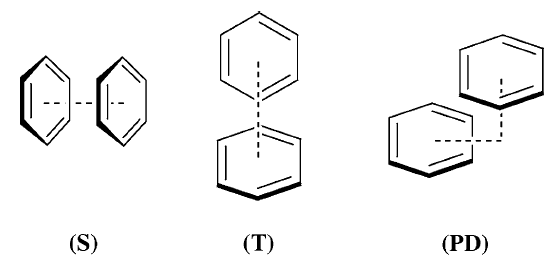
\includegraphics[scale=0.8]{image/Prot} \label{figprot}
 \caption[Structures du dimère de Benzène]{Structures des dimères de Benzène : (S) Sandwich, (T) En forme de T et (PD) Parallèle Déplacé}
 \end{figure}
 
 La stabilité relative entre la configuration en forme de T et la parallèle déplacée a été un sujet de nombreux études.
 
 La configuration en sandwich ayant une superposition maximal, peut apparaitre comme la plus favorable pour maximiser les interactions de dispersion, mais elle est rarement observée dans des systèmes contenant des noyaux phenyles, alors la configuration parallèle déplacée est souvent observée dans les structures cristallines de composés aromatiques \cite{hunter1991pi,fyfe1997synthetic,rebek1996assembly} ou dans les interactions des chaînes latérales aromatiques dedans les protéines \cite{hunter1991pi,burley1985aromatic}.\\
 
 Klemperer et al \cite{janda1975benzene} rapportent la configuration en forme de T comme prédominante dans leur étude de la molecule en phase gaz, ensuite du spectre rotationnel d'Arunan et Gutowsky \cite{arunan1993rotational}, en concordance avec Henson et al \cite{henson1992raman} qui rapportent par un étude de spectroscopie Raman que le dimère du benzène présente deux non équivalents monomères, un de bas et l'autre de symétrie élevée.\\ 
 
 Les calcules ab initio indiquent que las configurations (T) et (PD) présentent une barrière énergétique minimal de 0.1 kcal/mol \cite{park2006accurate}. Dans la littérature il existe considérables données pour l'énergie d'interaction du dimère de benzène, le tableau \ref{benzene} fournit un petit résume avec les valeurs obtenue par CCSD(T), en ce qui concerne à cette thèse, nous faisons attention aux interactions dans systèmes qui se présentent à l'état solide, par conséquent nous évaluons la méthode DFT-SAPT sur le système du benzène avec la configuration (PD), puisque cela expose des interaction $\pi$-stacking.
 
 \begin{table}[H]
 	\caption{Energie d'interaction du dimère de Benzène avec CCSD(T) en kcal/mol et DFT-SAPT (PBE0)}
 \begin{center}
 	 \begin{tabular}{l c c c c}
 	 	\toprule
 	& & T& & PD\\
 	\midrule
 	Park et Lee$^{1}$ & & -2,67& &-3,03\\
 	Tsuzuki et al$^{2}$ & & -2,46& & -2,48\\
 	Sinnokrot et al$^{3}$ & & -2,74& & -2,78\\
 	Hobza et al$^{4}$ & & -2,17& & -2,01\\
 	DFT-SAPT (PBE0) & & & & -2.35\\
 	\bottomrule
 \end{tabular}
\end{center}
\centering
\footnotemark[1]{ref \cite{park2006accurate}},
\footnotemark[2]{ref \cite{tsuzuki2002origin}},
\footnotemark[3]{ref \cite{sinnokrot2002estimates}},
\footnotemark[4]{ref \cite{hobza1996potential}}
\label{benzene}
\end{table}

La méthode DFT-SAPT donnée un valeur qui corresponde assez bien avec les resultats obtenus par CCSD(T) avec différents conditions de calculs. Pour cela nous proposons cette méthode pour l'étude des interaction dans les heterocycles aromatiques d'intérêt pour ce travail.  
     
 